%=======================02-713 LaTeX template, following the 15-210 template==================
%
% You don't need to use LaTeX or this template, but you must turn your homework in as
% a typeset PDF somehow.
%
% How to use:
%    1. Update your information in section "A" below
%    2. Write your answers in section "B" below. Precede answers for all 
%       parts of a question with the command "\question{n}{desc}" where n is
%       the question number and "desc" is a short, one-line description of 
%       the problem. There is no need to restate the problem.
%    3. If a question has multiple parts, precede the answer to part x with the
%       command "\part{x}".
%    4. If a problem asks you to design an algorithm, use the commands
%       \algorithm, \correctness, \runtime to precede your discussion of the 
%       description of the algorithm, its correctness, and its running time, respectively.
%    5. You can include graphics by using the command \includegraphics{FILENAME}
%
\documentclass[11pt]{article}
\usepackage{amsmath,amssymb,amsthm}
\usepackage{graphicx}
\usepackage[margin=1in]{geometry}
\usepackage{fancyhdr}
\setlength{\parindent}{0pt}
\setlength{\parskip}{5pt plus 1pt}
\setlength{\headheight}{13.6pt}
\newcommand\question[2]{\vspace{.25in}\hrule\textbf{#1: #2}\vspace{.5em}\hrule\vspace{.10in}}
\renewcommand\part[1]{\vspace{.10in}\textbf{(#1)}\par}
\newcommand\algorithm{\vspace{.10in}\textbf{Algorithm: }}
\newcommand\correctness{\vspace{.10in}\textbf{Correctness: }}
\newcommand\runtime{\vspace{.10in}\textbf{Running time: }}
\pagestyle{fancyplain}
\lhead{\textbf{\NAME}}
\chead{\textbf{{\COURSE} HW\HWNUM}}
\rhead{\today}
\begin{document}\raggedright
%Section A==============Change the values below to match your information==================
\newcommand\NAME{Eric Altenburg}  % your name
\newcommand\COURSE{CS-383}
\newcommand\HWNUM{3}              % the homework number
%Section B==============Put your answers to the questions below here=======================

% no need to restate the problem --- the graders know which problem is which,
% but replacing "The First Problem" with a short phrase will help you remember
% which problem this is when you read over your homework's to study.

\textit{\textbf{Pledge:} I pledge my honor that I have abided by the Stevens Honor System.} -Eric Altenburg

\question{4.3}{Page 369}
	\part{4.3.1}
		LDUR and STUR use the data memory resulting in \textbf{35\%}.\par
		
	\part{4.3.2}
		All instructions need to be fetched from instruction memory. Therefore, all types of instructions use instruction memory to reside and be fetched from. \textbf{100\%}.\par
		
	\part{4.3.3}
		The LDUR and STUR use sign-extension for the address offset. I-type has a 12-bit immediate value that needs to be zero-extended. Compare and Branch use a 19-bit field which needs to be extended to 64-bit address. Therefore, the total fraction of instructions includes \textbf{76\%}.\par
		
	\part{4.3.4}
		Although it is computed every cycle, when the sign-extended is not used, it is neglected since only 76\% of the total amount of instructions will utilize it.\par
		
		
\question{4.5}{Page 369}
	
	After converting to binary, the hex becomes: \par
	\begin{tabular}{c c c c c c c c}
		1111 & 1000 & 0000 & 0001 & 0100 & 0000 & 0110 & 0010
	\end{tabular}\par
	The op code is 11111000000 (bits 31-21).\par
	This converted to decimal is 1984 which in hex is 7C0.\par
	From this we can conclude that it is a D-type instruction.\par
	000010100 is the offset (bits 20-12).\par
	00 is the op (bits 11-10).\par
	00011 is the Rn (bits 9-5).\par
	00010 is the Rt (bits 4-0).\par
		
	\part{4.5.1}
		After moving through the sign extended, the output is:\par
		
		\begin{tabular}{c c c c c c c c c c c c c c c c}
			0000&0000&0000&0000&0000&0000&0000&0000&0000&0000&0000&0000&0000&0000&0001&0100
			%0000 & 0000 & 0000 & 0000 & 0100 & 0000 & 0110 & 0010
		\end{tabular}\par
		Output of the "shift left 2":\par
		\begin{tabular}{c c c c c c c c c c c c c c c c}
			0000&0000&0000&0000&0000&0000&0000&0000&0000&0000&0000&0000&0000&0000&0101&0000
			%0000 & 0000 & 0101& 0000 & 0001 & 1000 & 1000
		\end{tabular}\par
	
		
	\part{4.5.2}
%		ALU control process data is 100010 (0-5 bits). \par
%		$34_{10}$ or in hex $22$.\par
%		ALU main control operation is 111110 (26-32 bits).\par
%		$62_{10}$ or in hex $3E$.\par
		The value of the ALU control unit's input for this instruction is 0010.\par
		
	\part{4.5.3}
		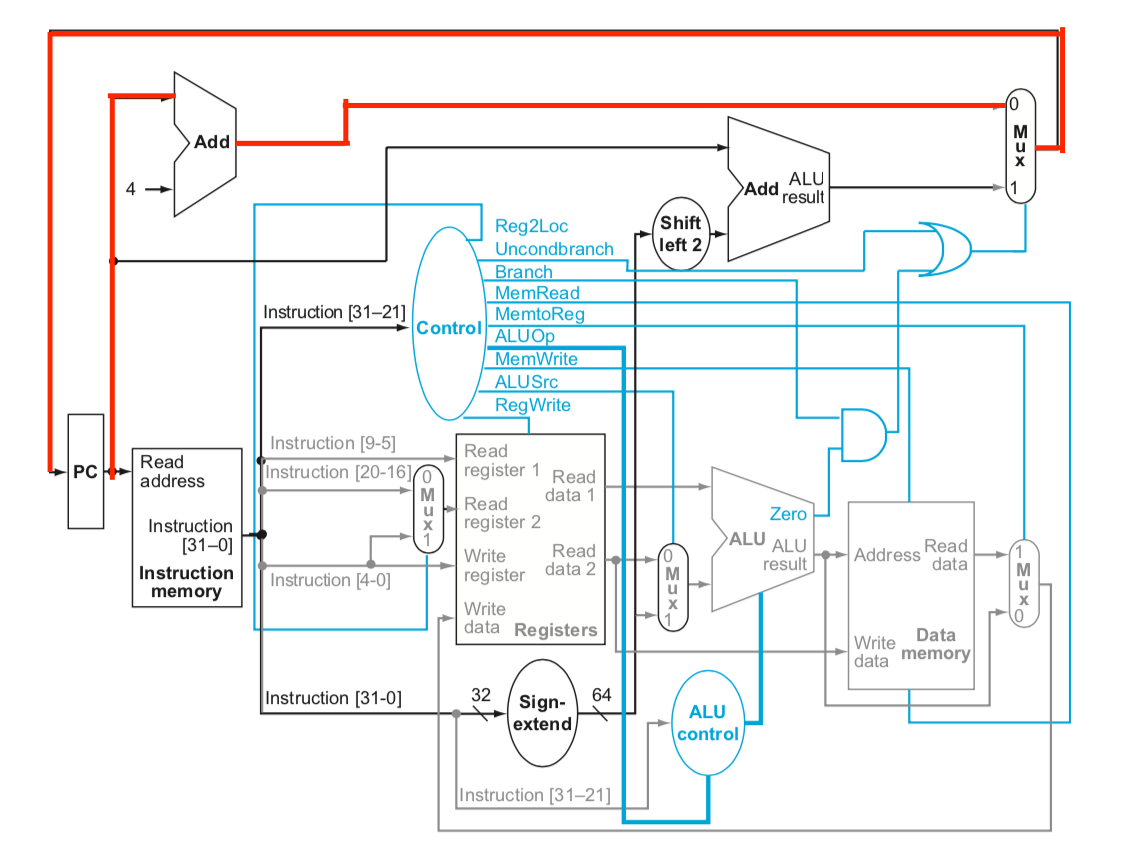
\includegraphics[scale=0.75]{images/453.png}\par
		After following the highlighted path in red, 4 gets added making the new PC address \textbf{PC+4}.\par
	
	
%
% Need to find out what to compare it to
%
\question{4.8}{Page 371}
	Assume for this problem an RType/IType takes 725 ps, LDUR takes 925 ps, STUR takes 880 ps, CBZ takes 735 ps, and B takes 525 ps.\par
	$CPU_{new} = (0.52*725)+(0.25*925)+(0.1*880) + (0.11*735)+(0.02*525)=\textbf{787.6}$ \textbf{ps}\par
	$CPU_{old} = 930 \; ps$\par
	$Speedup = \frac{930}{787.6}=1.18$ or an increase of \textbf{18\%}.
	
	
\question{4.9}{Page 371}
	For this problem, assume the clock cycles is 925 ps.\par
	\part{4.9.1}
		Without the multiplier, the clock cycle time would be \textbf{925 ps}.\par
		With the multiplier, the added 300 ps latency would result in a clock cycle time of \textbf{1225 ps}.\par
	
	\part{4.9.2}
		$Speedup_{new}=\frac{1}{0.95} * \frac{925ps}{1225ps}=$ \textbf{79.5\%}.\par
		This is not actually a speedup, instead, it is a decrease in performance as the clock cycle time increased after adding in the multiplier.\par
		
	\part{4.9.3}
		$(925+x) * 0.95 < 925$\par
		$x < 48.68$ ps\par
		Although the new CPU has 5\% fewer instructions, at most the new cycle time can add 48.68 ps to the ALU latency. However, from the problem, it instead adds 300 ps, therefore, the new ALU unit cannot be any slower and still result in an increase in performance.\par
	
	
\question{4.16}{Page 373}
	\part{4.16.1}
		Pipelined: Slowest of the times which is \textbf{350 ps}.\par
		Non-Pipelined: Each instruction is completed so adding them up gets us a clock cycle time of \textbf{1250 ps}.\par
	
	\part{4.16.2}
		Pipelined: Since it takes 5 cycles, $5*350=$ \textbf{1750 ps}.\par
		Non-pipelined: Just like the previous part, you would add up the times for each stage so \textbf{1250 ps}.\par
		
	\part{4.16.3}
		In choosing which stage to split, one should consider splitting the longest one which will then change the longest stage. The old longest stage, found in 4.16.1, was \textbf{350 ps}. The new longest stage after splitting up the aforementioned stage is \textbf{MEM at 300 ps}.\par
		
	\part{4.16.4}
		Since the data portion of the memory is only accessed by LDUR and STUR, the percentage of the clock cycles is only comprised of these two instructions which is \textbf{35\%}.
		
	
\question{4.18}{Page 374}
%	\begin{tabular}{|c|c|c|c|c|c|c|c|c|c|c|}
%		\hline
%		CC & 1 & 2 & 3 & 4 & 5 & 6 & 7 & 8 & 9 & 10\\
%		\hline
%		ADDI X1, X2, \#5 & IF & ID & EX & ME & WB & & & & &\\
%		\hline
%		ADD X3, X1, X2 & & IF & S & S & S & ID & EX & ME & WB & \\
%		\hline
%		ADDI X4, X1, \#15 & & & & & & IF & ID & EX & ME & WB\\
%		\hline
%	\end{tabular}\par

	\begin{tabular}{|c|c|c|c|c|c|c|c|c|}
		\hline
		CC & 1 & 2 & 3 & 4 & 5 & 6 & 7\\
		\hline
		ADDI X2, X2, \#5 & IF & ID & EX & ME & WB & &\\
		\hline
		ADD X3, X1, X2 & & IF & ID & EX & ME & WB&\\
		\hline
		ADDI X4, X1, \#15 & & & IF & ID & EX & ME & WB\\
		\hline
	\end{tabular}\par
	X3 = 33\par
	X4 = 26\par
	
\question{4.20}{Page 374}
	\begin{tabular}{c c c c}
		ADDI & X1, & X2, & \#5\\
		NOP & & & \\
		NOP & & & \\
		ADD & X3, & X1, & X2\\
		ADDI & X4, & X1, & \#15\\
		NOP & & & \\
		ADD & X5, & X3, & X2
	\end{tabular}

\question{4.22}{Page 375}
	\part{4.22.1}
		In order to fit the table on the page, I am assigning each instruction to the variables A, B, C, D, E, and F respectively. Also, NOP will be N in the table.\par
		\resizebox{16cm}{!}{
		\begin{tabular}{|c|c|c|c|c|c|c|c|c|c|c|c|c|c|c|c|c|c|c|c|c|c|}
			\hline
			CC & 1 & 2 & 3 & 4 & 5 & 6 & 7 & 8 & 9 & 10 & 11 & 12 & 13 & 14 & 15 & 16 & 17 & 18 & 19 & 20 & 21\\
			\hline
			A & IF & ID & EX & ME & WB &&&&&&&&&&&&&&&&\\
			\hline
			B & & IF& N & N & N & ID & EX & ME & WB &&&&&&&&&&&&\\
			\hline
			C & &  & IF& N & N & N & N & ID & EX & ME & WB &&&&&&&&&&\\
			\hline
			D & & & & IF& N & N & N & N & N & N & N & ID & EX & ME & WB &&&&&&\\
			\hline
			E & & & & & IF& N & N & N & N & N & N & N & N & ID & EX & ME & WB &&&&\\
			\hline
			F & & & & & & IF& N & N & N & N & N & N & N & N & N & N & N & ID & EX & ME & WB\\
			\hline
		\end{tabular}
		}\par
	\part{4.22.2}
		It is possible to rearrange the code in order to reduce the number of stalls by putting putting second line after the third line.\par
	
\question{4.25}{Page 376}
	\part{4.25.1}
		\resizebox{16cm}{!}{
		\begin{tabular}{|c|c|c|c|c|c|c|c|c|c|c|c|c|c|c|c|c|}
			\hline
			CC & 1 & 2 & 3 & 4 & 5 & 6 & 7 & 8 & 9 & 10 & 11 & 12 & 13 & 14 & 15 & 16\\
			\hline
			LDUR & IF & ID & EX & ME & WB &&&&&&&&&&&\\
			\hline
			LDUR & & IF & ID & EX & ME & WB &&&&&&&&&&\\
			\hline
			ADD & & & IF & Stall & ID & EX & ME & WB &&&&&&&&\\
			\hline
			SUBI & & & & & IF & ID & EX & ME & WB &&&&&&&\\
			\hline
			CBNZ & & & & & & IF & ID & EX & ME & WB &&&&&&\\
			\hline
			LDUR & & & & & & & IF & ID & EX & ME & WB &&&&&\\
			\hline
			LDUR & & & & & & & & IF & ID & EX & ME & WB &&&&\\
			\hline
			ADD & & & & & & & & & IF & Stall & ID & EX & ME & WB &&\\
			\hline
			SUBI & & & & & & & & & & & IF & ID & EX & ME & WB &\\
			\hline
			CBNZ & & & & & & & & & & & & IF & ID & EX & ME & WB\\
			\hline
		\end{tabular}
		}
	
\question{4.27}{Page 378}
	\part{4.27.1}
		\begin{tabular}{c c c c}
			ADD & X5, & X2, & X1\\
			NOP & & & \\
			NOP & & & \\
			LDUR & X3, & $[$X5, & \#4$]$\\
			LDUR & X2, & $[$X2, & \#0$]$\\
			NOP & & & \\
			ORR & X3, & X5, & X3\\
			NOP & & & \\
			NOP & & & \\
			STUR & X3, & $[$X5, & \#0$]$
		\end{tabular}

	\part{4.27.2}
		Even after attempting to rearrage the above code, the amount of NOP instructions remain the same. A reason for this, is because the instructions are dependent on the order in which they execute, therefore, one cannot rearrange the code.\par
	
	\part{4.27.3}
		If the processor has forwarding but with no hazard detection, when the code is being run, with forwarding you need the hazard system to detect problems, and without it, it won't be able to run because errors will run rampant because of hazards.\par
		
		
\question{4.29}{Page 379}
	\part{4.29.1}
		With the provided branch outcomes of T, NT, T, T, NT we can assess the following for the case where it is always-taken and always-not-taken: \par
		In the case where the predictors become T, T, T, T, T, there are only 3 out of the 5 that are correct, therefore, the accuracy is \textbf{$\frac{3}{5}$ or $60\%$}.\par
		
		In the case where the predictors become NT, NT, NT, NT, NT, there are only 2 out of the 5 that are correct, therefore, the accuracy is \textbf{$\frac{2}{5}$ or $40\%$}.\par 
	
	\part{4.29.2}
		\begin{enumerate}
			\item The first branch will result in a T, moving from strong predict not taken to weak predict not taken. Predicted outcome is not taken. The predictor value is 0.
			\item The second branch will result in a NT, moving from the weak predict not taken back to the strong predict not taken. Predicted outcome is not taken. The predictor value is 1.
			\item The third branch will result in a T, moving from strong predict not taken to weak predict not taken. Predicted outcome is not taken. The predictor value is 0.
			\item The forth branch will result in a T, moving from weak predict not taken to weak predict taken. Predicted outcome is not taken because it started out in the weak predict not taken. The predictor value is 0.
		\end{enumerate}
		After looking at the 4 outcomes, only 1 of them were correct (second branch) so the accuracy is \textbf{25\%}.

\end{document}